\documentclass{article}

\usepackage{titlesec}
\usepackage{titling}
\usepackage{graphicx}
\graphicspath{ {writeupimages/} }
\usepackage{float}

\titleformat{\section}
{\Large\bfseries}
{}
{0em}
{}[\titlerule]

\titleformat{\subsection}
{\large\bfseries}
{}
{0em}
{}

\titleformat{\subsubsection}
{\bfseries}
{}
{0em}
{}


\begin{document}

\title{Project: Perception Pick \& Place}
\author{Brett Gleason}

\maketitle

The rubric for this project can be found at the following URL: \\
https://review.udacity.com/\#!/rubrics/1067/view \\
I will consider the rubric points individually and describe how I addressed each point in my implementation.

\subsubsection{Required Steps for a Passing Submission:}

\begin{enumerate}
    \item Extract features and train an SVM model on new objects (see `pick\_list\_*.yaml` in `/pr2\_robot/config/` for the list of models you'll be trying to identify). 
    \item Write a ROS node and subscribe to `/pr2/world/points` topic. This topic contains noisy point cloud data that you must work with.
    \item Use filtering and RANSAC plane fitting to isolate the objects of interest from the rest of the scene.
    \item Apply Euclidean clustering to create separate clusters for individual items.
    \item Perform object recognition on these objects and assign them labels (markers in RViz).
    \item Calculate the centroid (average in x, y and z) of the set of points belonging to that each object.
    \item Create ROS messages containing the details of each object (name, pick\_pose, etc.) and write these messages out to `.yaml` files, one for each of the 3 scenarios (`test1-3.world` in `/pr2\_robot/worlds/`).  See the example `output.yaml` for details on what the output should look like.  
    \item Submit a link to your GitHub repo for the project or the Python code for your perception pipeline and your output `.yaml` files (3 `.yaml` files, one for each test world).  You must have correctly identified 100\% of objects from `pick\_list\_1.yaml` for `test1.world`, 80\% of items from `pick\_list\_2.yaml` for `test2.world` and 75\% of items from `pick\_list\_3.yaml` in `test3.world`.
    \item Congratulations!  You're done!
\end{enumerate}



% # Extra Challenges: Complete the Pick & Place

% 7. To create a collision map, publish a point cloud to the `/pr2/3d_map/points` topic and make sure you change the `point_cloud_topic` to `/pr2/3d_map/points` in `sensors.yaml` in the `/pr2_robot/config/` directory. This topic is read by Moveit!, which uses this point cloud input to generate a collision map, allowing the robot to plan its trajectory.  Keep in mind that later when you go to pick up an object, you must first remove it from this point cloud so it is removed from the collision map!

% 8. Rotate the robot to generate collision map of table sides. This can be accomplished by publishing joint angle value(in radians) to `/pr2/world_joint_controller/command`

% 9. Rotate the robot back to its original state.

% 10. Create a ROS Client for the “pick_place_routine” rosservice.  In the required steps above, you already created the messages you need to use this service. Checkout the [PickPlace.srv](https://github.com/udacity/RoboND-Perception-Project/tree/master/pr2_robot/srv) file to find out what arguments you must pass to this service.

% 11. If everything was done correctly, when you pass the appropriate messages to the `pick_place_routine` service, the selected arm will perform pick and place operation and display trajectory in the RViz window

% 12. Place all the objects from your pick list in their respective dropoff box and you have completed the challenge!

% 13. Looking for a bigger challenge?  Load up the `challenge.world` scenario and see if you can get your perception pipeline working there!


---
\section{Writeup / README}

\subsection{1. Provide a Writeup / README that includes all the rubric points and how you addressed each one.  You can submit your writeup as markdown or pdf.}

You're reading it!

\section{Exercise 1, 2 and 3 pipeline implemented}
\subsection{1. Complete Exercise 1 steps. Pipeline for filtering and RANSAC plane fitting implemented.}
The objective of exercise 1 was to take a simulated scene with several objects on a table and create two separate point cloud files: the first containing the table surface and the second containing the objects on the table. To accomplish this, several filters were used as well as the random sample consensus (or RANSAC) algorithm.

\begin{figure}[H]
    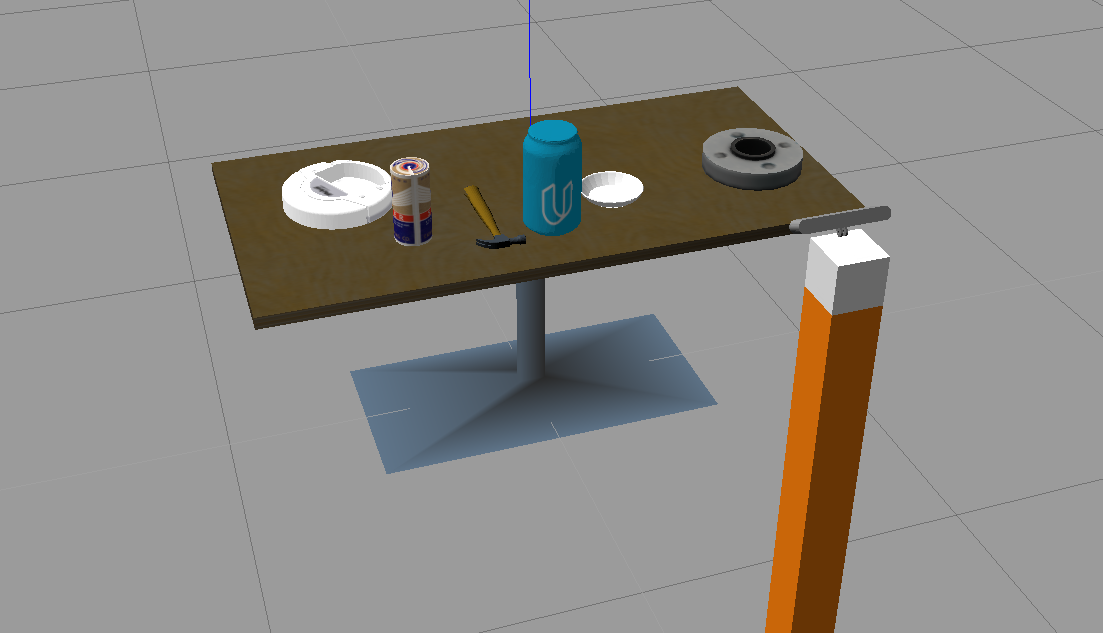
\includegraphics[width=\linewidth]{gazeboscene.png}
    \caption{Simulated environment in Gazebo with camera on sensor stick, objects on table}
    \label{fig:gazebo}
\end{figure}

\begin{figure}[H]
    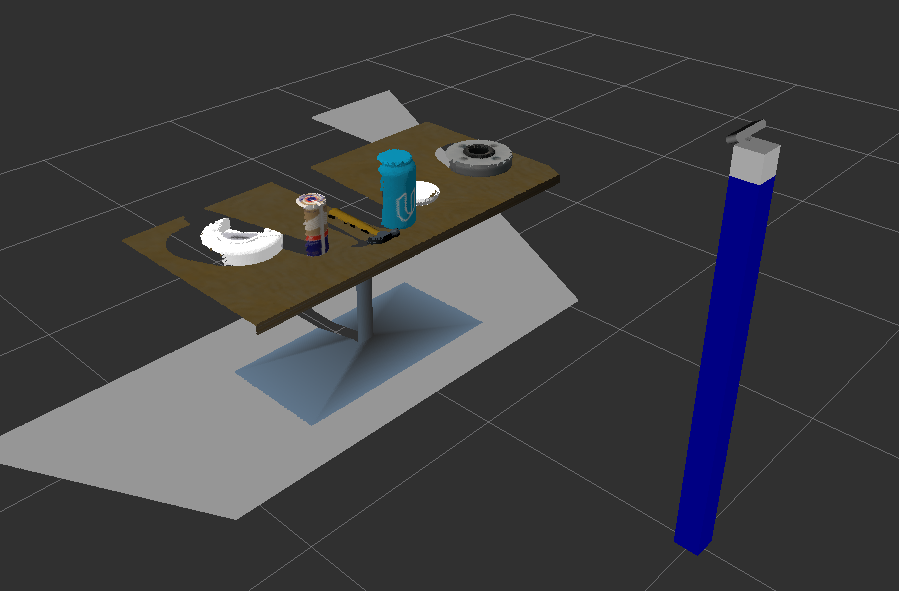
\includegraphics[width=\linewidth]{scene.png}
    \caption{Simulated environment in RViz with camera on sensor stick, objects on table}
    \label{fig:scene}
\end{figure}

\subsubsection{Voxel Grid Downsampling}
The starting point for this exercise is a point cloud file from a simulated RGB-D camera. The point cloud from the RGB-D camera is very dense, meaning any operations on it will be very computationally intense.

\begin{figure}[H]
    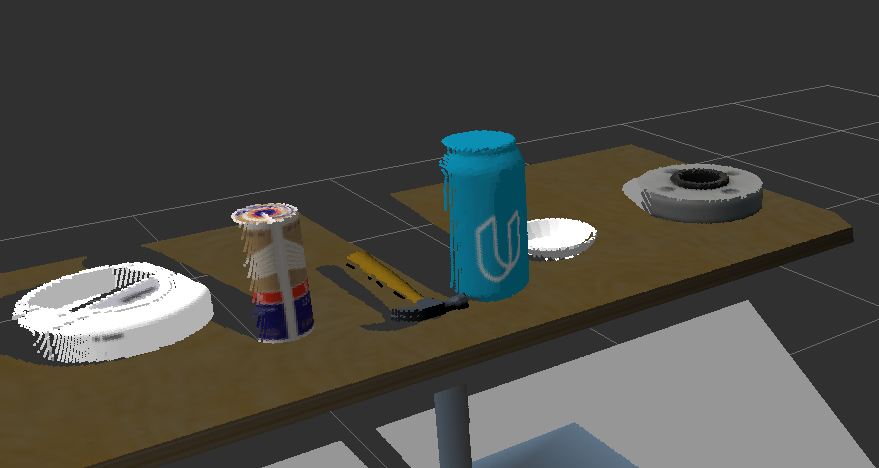
\includegraphics[width=\linewidth]{sspc.png}
    \caption{Point cloud file from RGB-D camera as shown in Rviz}
    \label{fig:Rvizcamera}
\end{figure}

\begin{figure}[H]
    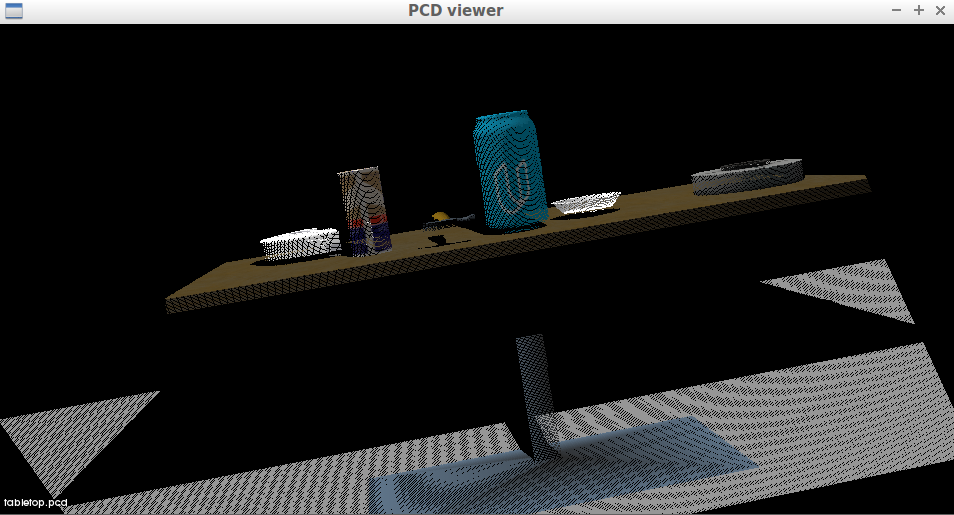
\includegraphics[width=\linewidth]{ex1tabletop.png}
    \caption{Point cloud file from RGB-D camera as shown in PCL viewer}
    \label{fig:camera}
\end{figure}

Voxel grid downsampling reduces the density of the point cloud, allowing for faster computations without any loss in the ability for the point cloud data to be used for object recognition later in the perception pipeline. A voxel can be thought of as a three dimensional analog to a pixel. The input point cloud can be divided into a voxel grid by dividing it into cubic regions. To perform the voxel grid downsampling, the points within each cubic region (voxel) are replaced with a single point that represents the average of the points contained within the voxel. By choosing the size of the voxel appropriately, the downsampled point cloud will provide a good approximation of the original point cloud while allowing faster computation in later steps.
For this project, voxel grid downsampling is accomplished using the python PCL library (Point Cloud Library). A VoxelGrid filter object is created from the input point cloud and a filter() function can be run on this object after the size of the voxel is set.

\begin{figure}[H]
    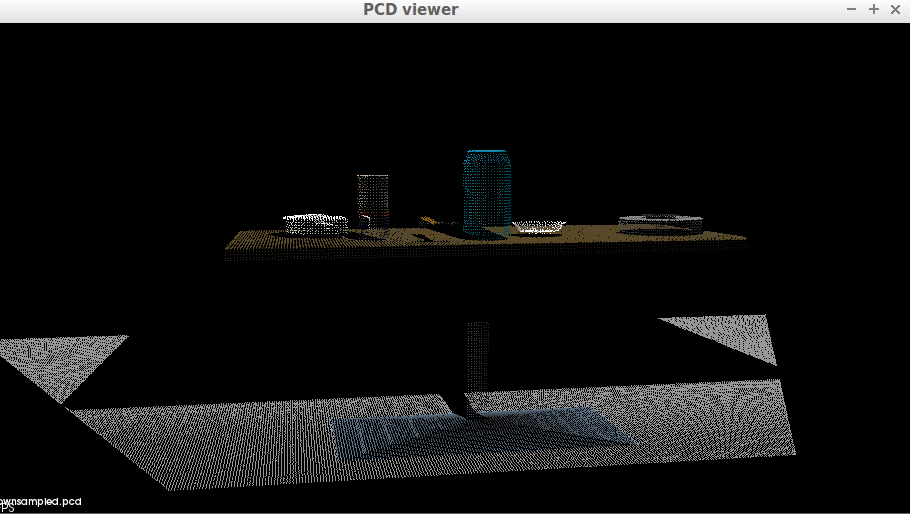
\includegraphics[width=\linewidth]{ex1downsampled.png}
    \caption{Point cloud file after voxel grid downsampling as shown in PCL viewer}
    \label{fig:downsampled}
\end{figure}

\subsubsection{Pass Through Filtering}
Because the robot and the table are both stationary for this project it is easy to filter out parts of the point cloud that are not relevant. For this exercise a region on the Z-axis was selected such that only the table and the objects on it would be able to "pass through" the filter as shown in figure \ref{fig:passthrough}.

\begin{figure}[H]
    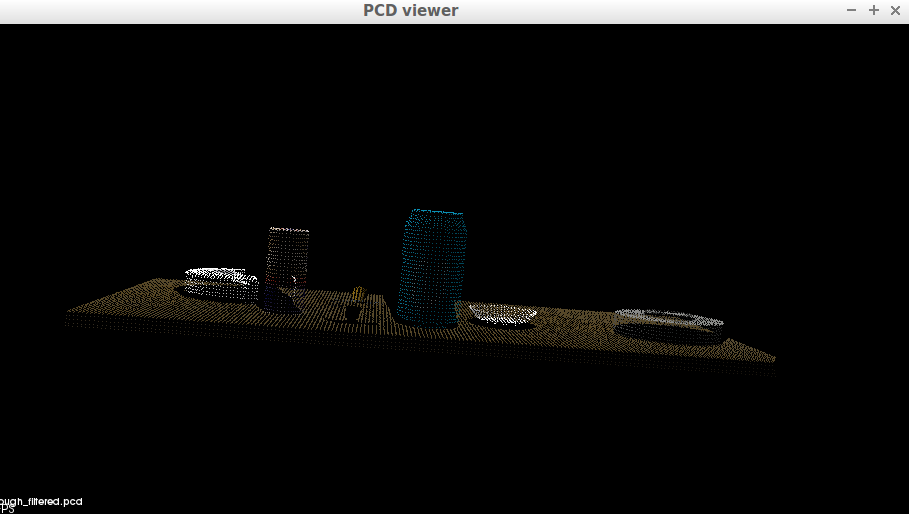
\includegraphics[width=\linewidth]{ex1passthrough.png}
    \caption{Point cloud file after pass through filtering as shown in PCL viewer}
    \label{fig:passthrough}
\end{figure}

\subsubsection{RANSAC}
Finally, random sample consensus (or RANSAC) is an algorithm that can be used to remove the table from the point cloud, leaving only the objects of interest behind. RANSAC determines whether each point in the cloud belongs to a particular model. If the point fits the model it is classified as an inlier, if it doesn't fit it is an outlier. For this exercise a plane was used as the model, resulting in the points belonging to the table being classified as inliers to the plane, while the points belonging to the objects on the table were classified as outliers. At this point the objective of the exercise is accomplished, the input point cloud from the RGB-D camera has been separated into a point cloud containing the table surface and a point cloud containing the objects of interest.

\begin{figure}[H]
    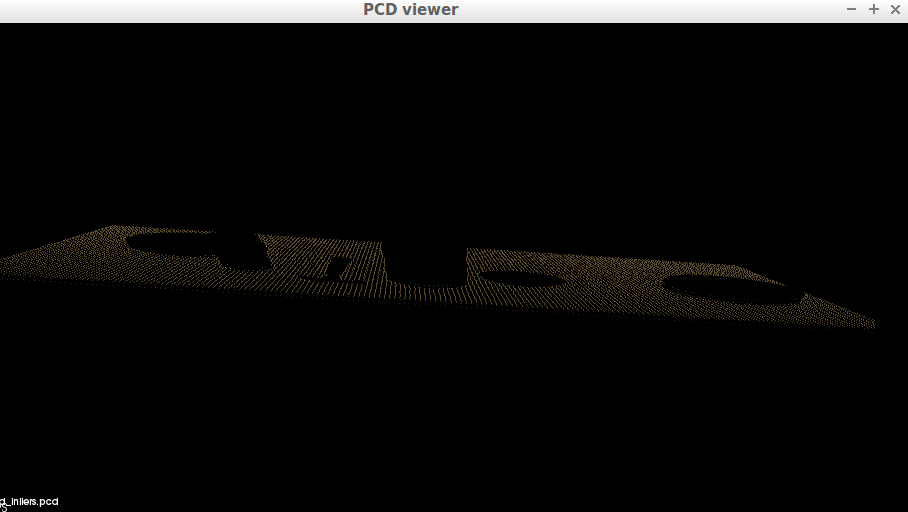
\includegraphics[width=\linewidth]{ex1extractedinliers.png}
    \caption{RANSAC inliers as shown in PCL viewer}
    \label{fig:inliers}
\end{figure}

\begin{figure}[H]
    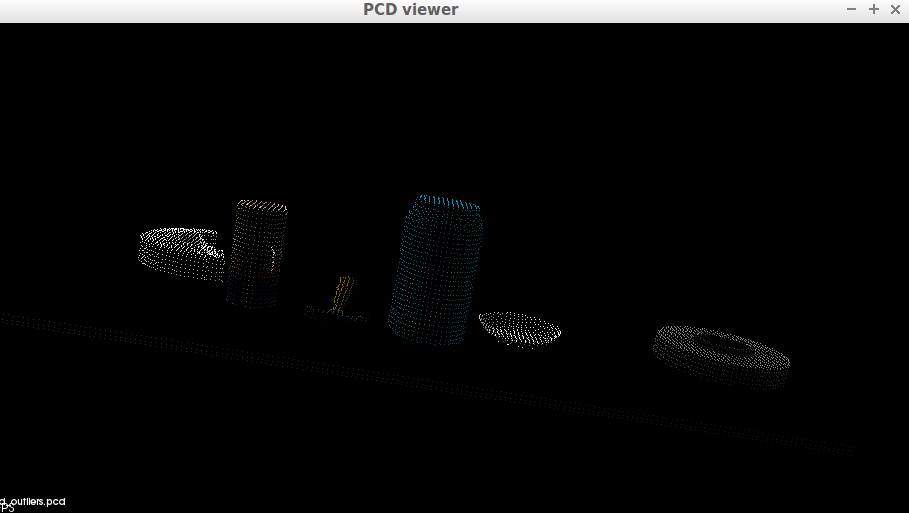
\includegraphics[width=\linewidth]{ex1extractedoutliers.png}
    \caption{RANSAC outliers as shown in PCL viewer}
    \label{fig:outliers}
\end{figure}

\subsection{2. Complete Exercise 2 steps: Pipeline including clustering for segmentation implemented.}
For the second exercise the objective was to take the filtered point cloud containing the objects as shown in figure \ref{fig:outliers} and use Euclidean clustering to segment the points belonging to each individual object. In this exercise an additional pass through filter along the Y-axis was added so that the edge of the table would be removed from the scene.

\subsubsection{Euclidean Clustering}
The Euclidean clustering algorithm requires that a k-dimensional tree (or k-d tree) be constructed from the input point cloud before the algorithm is run. A k-d tree is a type of binary search tree that allows a nearest neighbor search to be done efficiently. K-d trees are not the only data structure that can be used to efficiently perform a nearest neighbor seach and accomplish point cloud segmentation, but PCL's implementation of Euclidean Clustering requires a k-d tree.

Euclidean clustering segments the points in the point cloud into clusters based on several parameters:
\begin{itemize}
    \item Cluster tolerance
    \item Minimum cluster size
    \item Maximum cluster size
\end{itemize}

The cluster tolerance is the maximum distance that a point can have to its nearest neighbor and remain part of the cluster. Cluster tolerance needs to be set large enough that the points within each object are considered part of the cluster but small enough that the distance between two objects is not within the cluster tolerance, causing the two objects to become part of the same cluster.
Minimum cluster size is the minimum number of points needed to constitute a cluster. Minimum cluster size needs to be set large enough that noise in the data is not considered a cluster, but small enough that an actual cluster is not disqualified. 
Maximum cluster size is the maximum number of points that can constitute a cluster, it must be set large enough that none of the objects in the point cloud are disqualified.
Once the clustering parameters have been set appropriately, the Euclidean clustering algorithm can be applied to the point cloud. Figure \ref{fig:preec} shows the point cloud pre Euclidean clustering, while figure \ref{fig:ec} shows the point cloud post Euclidean clustering. The clusters are colorized during the clustering step for visual clarity.

\begin{figure}[H]
    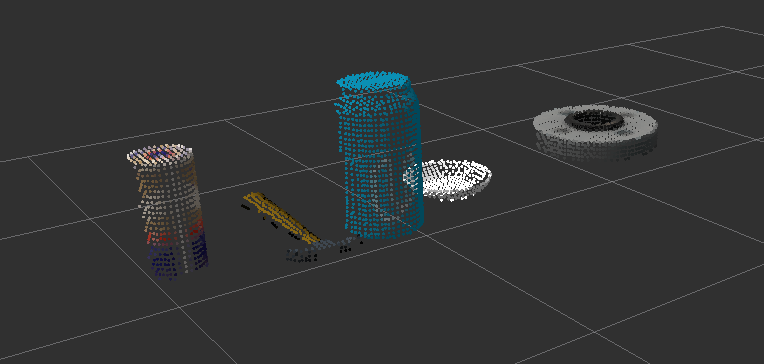
\includegraphics[width=\linewidth]{preec.png}
    \caption{RANSAC outliers pre Euclidean Clustering, as shown in RViz}
    \label{fig:preec}
\end{figure}

\begin{figure}[H]
    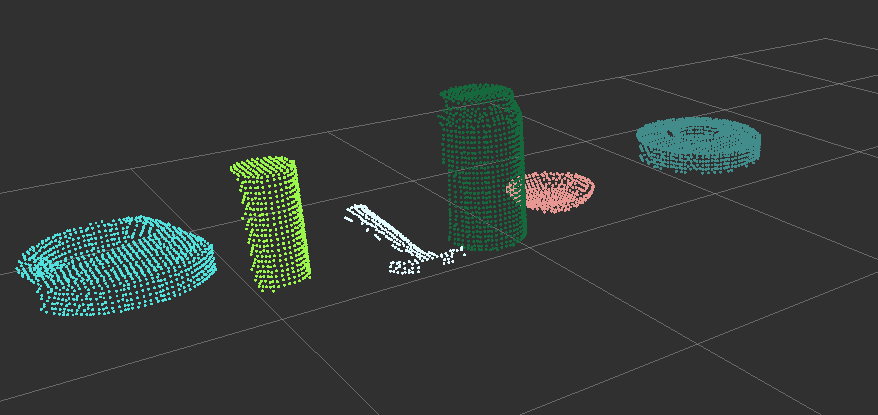
\includegraphics[width=\linewidth]{ec.png}
    \caption{Point cloud after Euclidean clustering, as shown in RViz}
    \label{fig:ec}
\end{figure}

\subsection{3. Complete Exercise 3 Steps.  Features extracted and SVM trained.  Object recognition implemented.}
In exercise-1 and 2 the input point cloud from the RGB-D camera was filtered and segmented, leaving only clusters of points belonging to the objects of interest. The goal of exercise 3 was to train a support vector machine to recognize the objects in the filtered and segmented point cloud.

\subsubsection{SVM}
A support vector machine (SVM) is a machine learning algorithm used to classify objects. The SVM is trained on a data set containing multiple objects, where each object consists of a feature vector and a label. The SVM maps the feature vectors and the labels and uses the training data to draw boundaries between the different objects in the dataset. Once these boundaries are drawn, a feature vector can be input to the model and it will be characterized and given a label based on which boundaries it falls between.

\begin{figure}[H]
    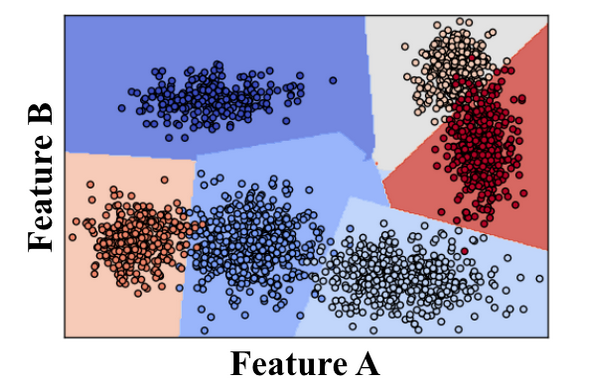
\includegraphics[width=\linewidth]{SVMexample.png}
    \caption{Example SVM data set}
    \label{fig:SVMex}
\end{figure}

Figure \ref{fig:SVMex} shows an example SVM data set based on two feature vectors, feature A and feature B. The feature vectors are grouped into clusters and then boundaries are drawn between the clusters to separate them into classes. An additional object given to the SVM could now be classified based on where it falls within this dataset.

\subsubsection{Surface Normals and Color}
The feature vectors used for this exercise are the color and the surface normal vectors. For the color vector, 3 color channels are turned into histograms and concatenated, then normalized. Initially the 3 channels were RGB, but they were changed to HSV later to improve the model. The surface normal vector was calculated similarly to the color vector, except that instead of 3 color channels to make the histograms the X, Y, and Z components of the surface normal vectors were used. After the surface normal histograms are concatenated and normalized, the color and surface normal histograms can be concatenated to create the complete feature vector.

\subsubsection{SVM Training}
The SVM was trained by placing each object to be classified in a random pose for the camera. The features were extracted and used to assemble the training data set. Initially each object was placed in 5 random poses. Once the features had been generated, the python Scikit-learn package was used to train the SVM. To represent the accuracy of the SVM, a confusion matrix was created. The Y axis represents the actual instances of the object while the X axis represents the SVM's classified instances of the object. On the left is a confusion matrix with the raw counts, on the right is a confusion matrix with the counts normalized from 0-1. Figure \ref{fig:SVMinit} shows the confusion matrix for the first SVM.

\begin{figure}[H]
    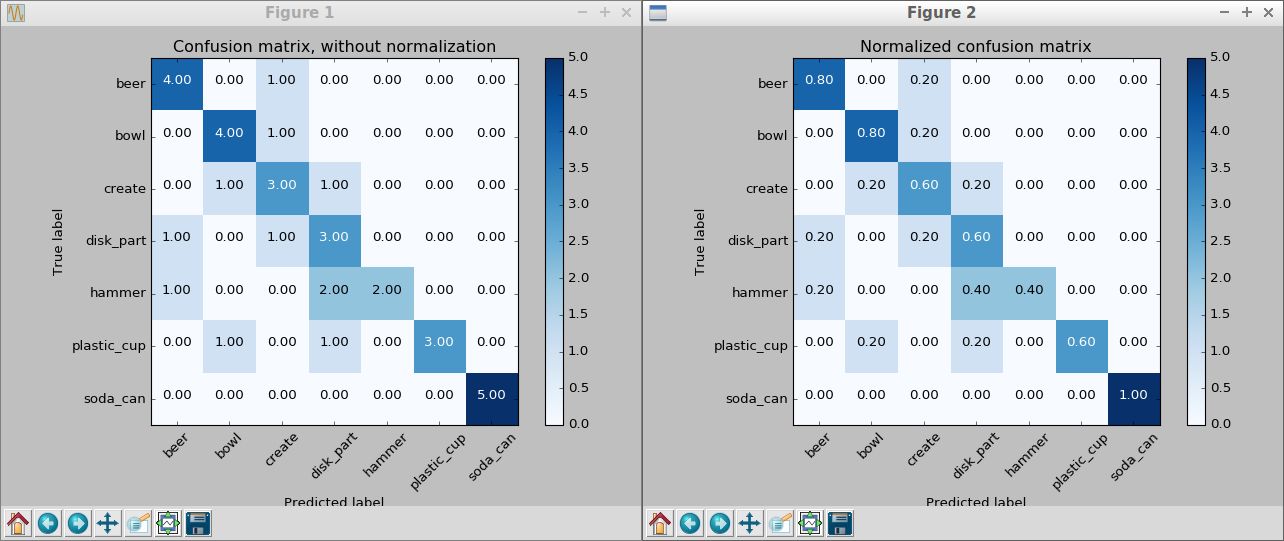
\includegraphics[width=\linewidth]{ex3SVMinitial.png}
    \caption{Confusion matrix for the first SVM}
    \label{fig:SVMinit}
\end{figure}

The initial result after training the SVM was not good enough to correctly identify the objects. The feature vector was changed to use HSV color space instead of RGB in an attempt to increase the accuracy of the SVM. Figure \ref{fig:SVMHSV} shows the results after generating features and re-training the SVM.

\begin{figure}[H]
    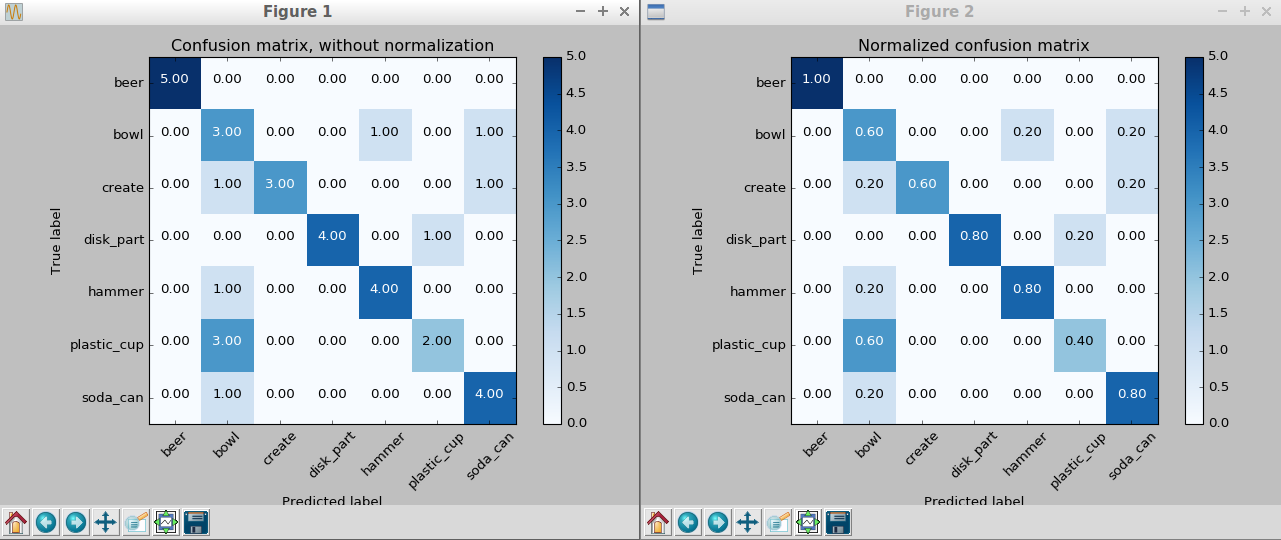
\includegraphics[width=\linewidth]{ex3SVMHSV.png}
    \caption{Confusion matrix using HSV color space instead of RGB}
    \label{fig:SVMHSV}
\end{figure}

After converting from RGB to HSV color vectors the SVM was still not accurate enough for object identification. The next step was to increase the number of poses for each object from 5 to 25 for the feature generation. Figure \ref{fig:SVM25} shows the results of training the SVM with the additional feature data.

\begin{figure}[H]
    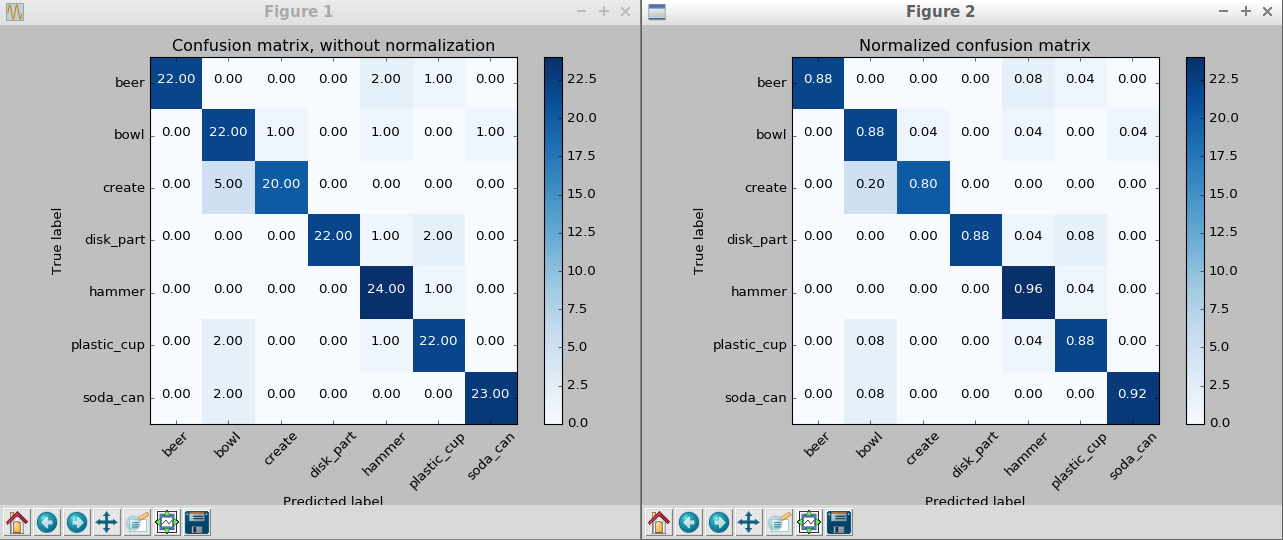
\includegraphics[width=\linewidth]{ex3SVM25.png}
    \caption{Confusion matrix after using 25 poses for each object for feature generation}
    \label{fig:SVM25}
\end{figure}

After this adjustment the SVM was accurate enough to correctly identify the objects on the table and exercise 3 was complete.

\begin{figure}[H]
    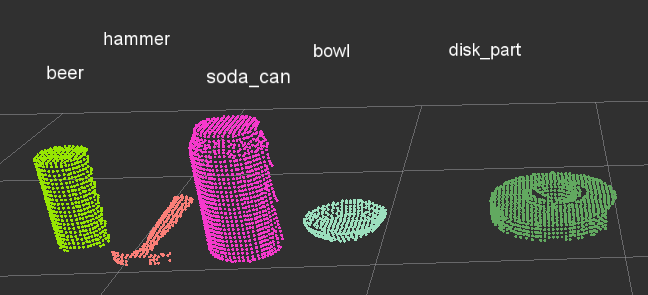
\includegraphics[width=\linewidth]{classification.png}
    \caption{Point cloud after clustering with object recognition applied. Shown in RViz.}
    \label{fig:classification}
\end{figure}

\section{Pick and Place Setup}

\subsection{1. For all three tabletop setups (`test*.world`), perform object recognition, then read in respective pick list (`pick\_list\_*.yaml`). Next construct the messages that would comprise a valid `PickPlace` request output them to `.yaml` format.}\label{subsec:projintro}

The project simulation is done with a PR2 robot from Willow Garage. The robot is presented with three different arrangements of items on the table. For a successful project the robot must get instructions on which items to pick from the pick\_list\_*.yaml file, find the object on the table, construct a 'PickPlace' request for each item in the scene and output the requests to a .yaml file. A PickPlace request is an assembly of multiple ROS messages containing the following information:
\begin{itemize}
    \item Test Scene Number - the number corresponding to the tabletop setup being used.
    \item Object Name - the label corresponding to the object to be picked.
    \item Arm Name - which of the robot's arms should be used for the pick/place operation for this object.
    \item Pick Pose - the position of the object to be picked.
    \item Place Pose - the position of the bin that the object should be placed into.
\end{itemize}

\begin{figure}[H]
    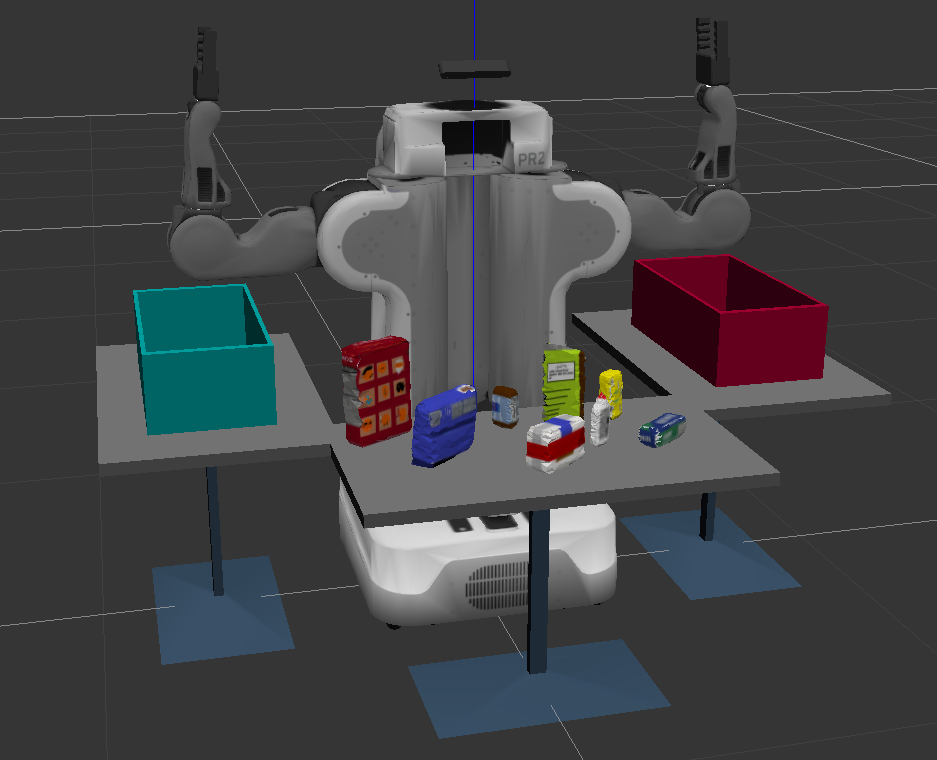
\includegraphics[width=\linewidth]{pr2.png}
    \caption{Project environment as shown in Gazebo. The third test environment is shown.}
    \label{fig:pr2}
\end{figure}

\subsubsection{Perception Pipeline - Filtering and Segmentation}
The filtering portion of the perception pipeline for the project was implemented similarly to exercise-1. An additional challenge introduced in the project is that the input from the RGB-D camera now contained noise.

\begin{figure}[H]
    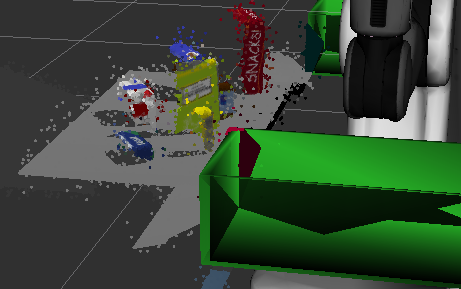
\includegraphics[width=\linewidth]{pr2noise.png}
    \caption{Noisy input from RGB-D camera.}
    \label{fig:noise}
\end{figure}

To remove the noise, a statistical outlier filter was used. In the outlier filter, the distance between each point and its neighboring points are considered. If the point under consideration is further away from its neighbors than the mean distance plus a multiple of the standard deviation of the mean distance, it is considered an outlier and removed. The PCL statistical outlier filter object was used to perform this filtration

After the statistical outlier filter, the filtration steps are very similar to the first exercise. Voxel grid downsampling was performed to increase computational speed. A passthrough filter was used to isolate the table and the objects. RANSAC plane fitting was used to separate the table and the objects into separate point clouds.

\begin{figure}[H]
    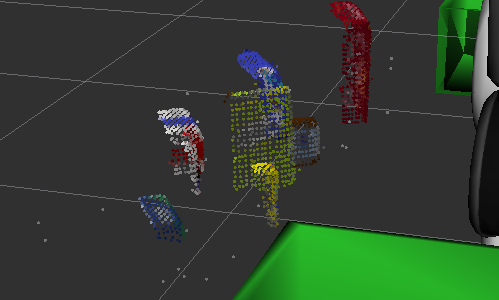
\includegraphics[width=\linewidth]{pr2objects.png}
    \caption{Table objects after the filtration steps have been performed.}
    \label{fig:pr2objects}
\end{figure}

Once the filtration step was complete, the point cloud was segmented using Euclidean clustering as in exercise-2.

\begin{figure}[H]
    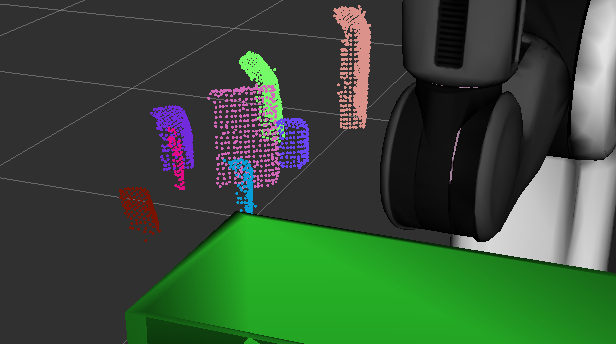
\includegraphics[width=\linewidth]{pr2cluster.png}
    \caption{Table objects after Euclidean clustering}
    \label{fig:pr2cluster}
\end{figure}

\subsubsection{Perception Pipeline - Object Recognition}
Object recognition was performed using a support vector machine as in exercise-3. The new test scenes contained different objects so the SVM needed to be retrained. I used 25 poses per object for the first attempt because it was successful in exercise-3. Figure \ref{fig:pr2SVM25} shows the confusion matrix after training the SVM with this data.

\begin{figure}[H]
    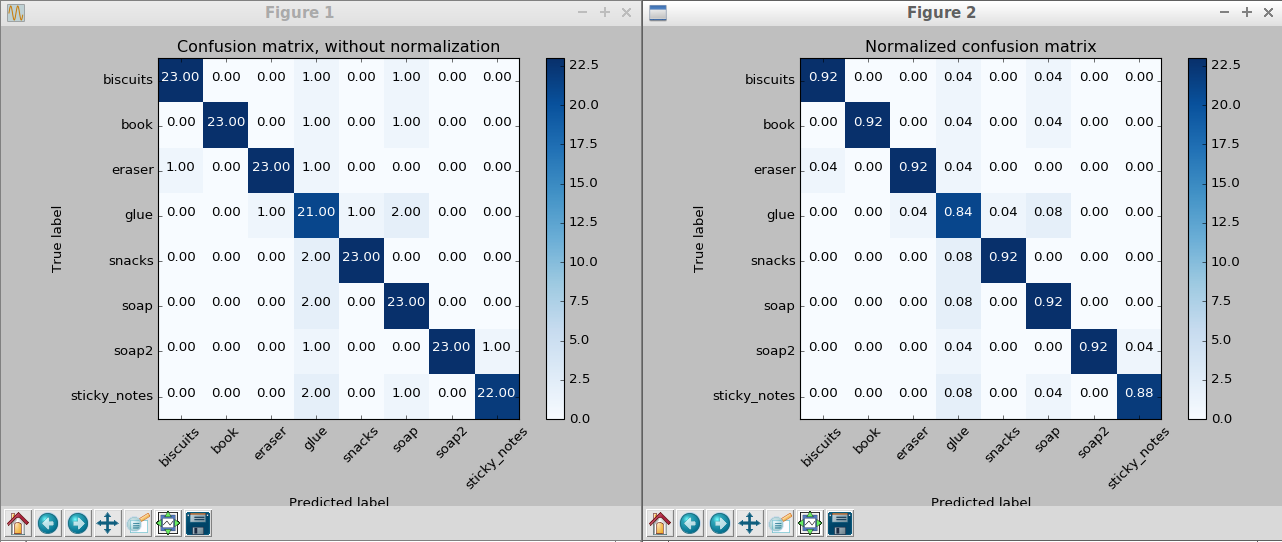
\includegraphics[width=\linewidth]{pr2SVM25.png}
    \caption{Confusion matrix for the SVM trained on 25 poses per object}
    \label{fig:pr2SVM25}
\end{figure}

Unfortunately the object recognition had too many errors when using this model. A second attempt was made using 50 poses per object.

\begin{figure}[H]
    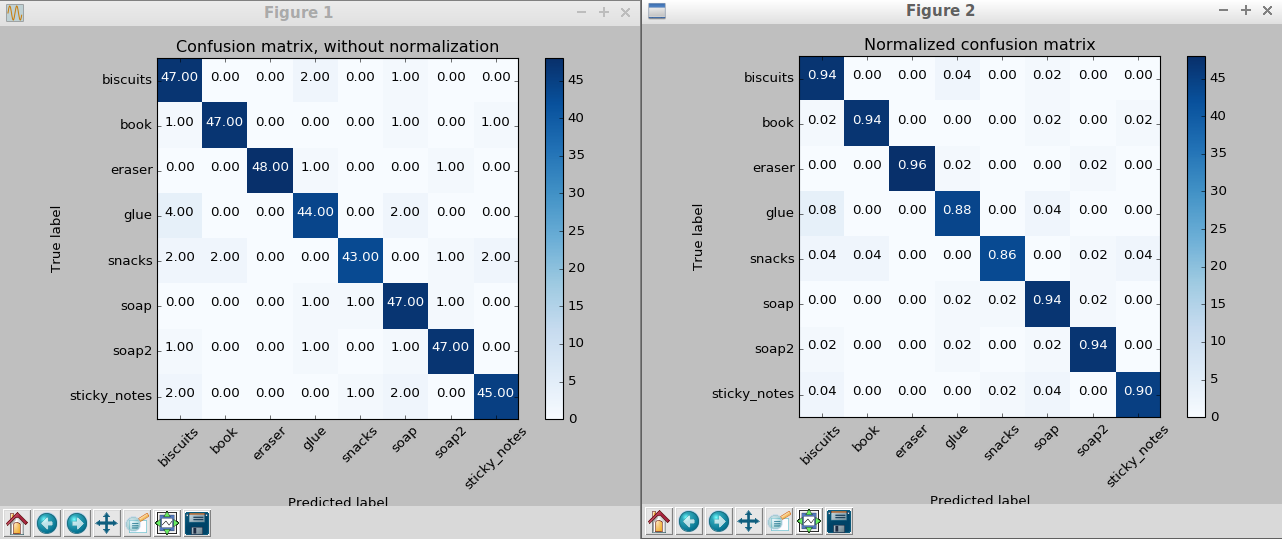
\includegraphics[width=\linewidth]{pr2SVM50.png}
    \caption{Confusion matrix for the SVM trained on 50 poses per object}
    \label{fig:pr2SVM50}
\end{figure}

Figure \ref{fig:pr2objrec} shows the results of the object recognition step using this model on the third test world.

\begin{figure}[H]
    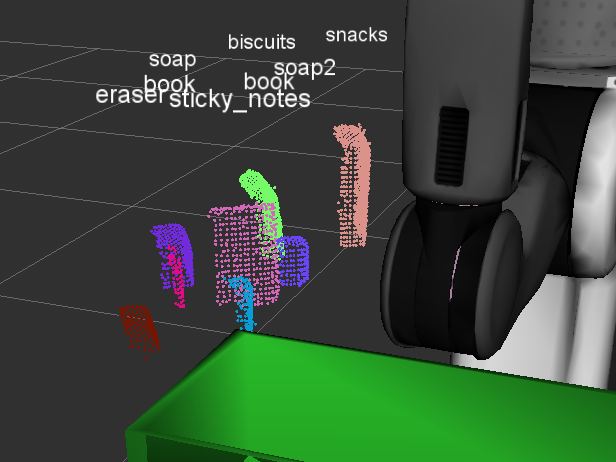
\includegraphics[width=\linewidth]{pr2objrec.png}
    \caption{Object recognition using an SVM trained on 50 poses per object}
    \label{fig:pr2objrec}
\end{figure}

\subsubsection{Create PickPlace Request}
Once the object recognition was working sufficiently well it was time to create the PickPlace request. Here are the components of a PickPlace request as detailed in section \ref{subsec:projintro}: test scene number, object name, arm name, pick pose, and place pose. Each of the three test worlds has a corresponding pick\_list.yaml file that was loaded into the ROS parameter server. The pick list details each object that is expected to be found in the test world and which bin it should be placed in.

The test scene number is derived from which test scene is loaded, it is the same for every item in the scene. The name for each item is listed on the pick list. The arm to be used for the pick and place operation is also determined by parsing the pick list. The pick list lists one of two groups for each item corresponding to the bins at the robots side: green corresponds to the bin on the right, while red corresponds to the group on the left. The arm name is assigned as either right or left to match the bin the item is to be placed in.

To determine the position of the item to be picked, the object name from the pick list must first be matched to a label given to one of the objects in the robot's field of view by the object detection step. Once the object is found, its centroid must be calculated. Using the point cloud for the detected object, the average position of the points along each axis is calculated and assigned as the X, Y, and Z positions of the pick pose.

Lastly, the position where the object should be placed can be determined. There are two possible positions for the place pose based on which bin the object is assigned to. The bin is already known from assigning the correct arm for the operation, all that is left is to parse the drop box positions. There is a dropbox.yaml file that was loaded into the ROS parameter server along with the pick list. Using the arm name the bin position can be parsed similarly to the pick list and the place pose can be found.

% Spend some time at the end to discuss your code, what techniques you used, what worked and why, where the implementation might fail and how you might improve it if you were going to pursue this project further.  


\end{document}
